% Provenance (never printed): sources/book2/BRIEFS.md, g10-02. Two goods, fixed resources;
% opportunity cost as a slope; the bowed frontier; moving the frontier. Real numbers from
% figdata/grade-10/02-production-possibility-frontier/ (JST Macrohistory Database); Brenland's
% valleys are invented and their numbers are given in the text.
\chapter{The Production Possibility Frontier}\label{ch:g10:production-possibility-frontier}

In September 1939 the United Kingdom went to war; in December 1941 the United States followed.
% ledger: g10:uk-war-1939, g10:us-war-1941
Both had to produce aircraft, ships, shells and uniforms in quantities never seen before, and both
did. What happened to everything else is the subject of the opening chart. In the United Kingdom,
output per person rose by about a quarter between 1939 and 1943, while consumption per person ---
food, clothing, fuel, everything households bought --- fell by about a sixth. In the United States,
output per person rose by four-fifths between 1939 and 1944, and consumption per person did not
fall at all: it rose by a tenth. The United States produced a war and more consumer goods at the same
time.
% figdata: war_gbr (1943: gdp_pp 123.7, cons_pp 83.5); war_usa (1944: gdp_pp 180.2, cons_pp 110)

The same war, two different costs. This chapter builds the simplest model that explains the
difference, the \omterm{def:g10:production-possibility-frontier:ppf}{production possibility frontier}, and uses it to give the old notion of opportunity
cost a shape and a number.

\begin{openingchart}{Real output (GDP) and real consumption per person, United States and United
Kingdom, 1929--1950, as indices with 1939 = 100. The shaded years are those of each country's war
(1939--1945 for the United Kingdom, 1941--1945 for the United States).}{Jord\`a--Schularick--Taylor
Macrohistory Database; real GDP per person and real consumption per person}
\begin{tikzpicture}
\begin{groupplot}[group style={group size=2 by 1, horizontal sep=1.3cm, y descriptions at=edge left},
  omtime, width=0.48\linewidth, height=6.4cm, xmin=1929, xmax=1950, ymin=60, ymax=200,
  xtick={1930,1935,...,1950}, ytick={60,80,...,200}, legend pos=north west]
\nextgroupplot[title={\small United States}, ylabel={index, 1939 = 100}]
\fill[black!7] (axis cs:1941,60) rectangle (axis cs:1945,200);
\addplot[omDef, thick] table[x=year, y=gdp_pp] {figdata/grade-10/02-production-possibility-frontier/out/war_usa.csv};
\addlegendentry{output}
\addplot[omThm, thick] table[x=year, y=cons_pp] {figdata/grade-10/02-production-possibility-frontier/out/war_usa.csv};
\addlegendentry{consumption}
\nextgroupplot[title={\small United Kingdom}]
\fill[black!7] (axis cs:1939,60) rectangle (axis cs:1945,200);
\addplot[omDef, thick] table[x=year, y=gdp_pp] {figdata/grade-10/02-production-possibility-frontier/out/war_gbr.csv};
\addplot[omThm, thick] table[x=year, y=cons_pp] {figdata/grade-10/02-production-possibility-frontier/out/war_gbr.csv};
\end{groupplot}
\end{tikzpicture}
\end{openingchart}

\begin{recall}
From the grades 6--9 volume: the \emph{opportunity cost} of a choice is the value of the best option
given up for it. The \emph{factors of production} --- labour, capital and natural resources --- are
combined with a technology to make goods and services; with a given quantity of each, output is
limited. From mathematics: a linear function $y = a - bx$ has a straight graph, and its slope $-b$
says by how much $y$ changes when $x$ rises by one.
\end{recall}

\section{Two goods and fixed resources}\label{sec:g10:production-possibility-frontier:two-goods}

A real economy produces millions of different goods. The model keeps two, or two groups: grain and
cloth, food and machines, consumer goods and military goods. It fixes the quantities of the factors
of production and the technology, for a period short enough that they do not change much, and asks
one question: which combinations of the two goods can be produced?

\begin{example}[The North Valley]\label{ex:g10:production-possibility-frontier:north}
In the North Valley of Brenland, an invented economy, the farms and workshops have \num{1200} hours of
work a week. A tonne of grain takes 3 hours of work and a roll of cloth 2 hours. If the valley
produces $G$ tonnes of grain and $C$ rolls of cloth a week, it uses $3G + 2C$ hours, and it cannot use
more than it has:
\[
  3G + 2C \le 1200 .
\]
Using every hour, $3G + 2C = 1200$, which gives $C = 600 - 1.5\,G$. With all hours on cloth the valley
makes 600 rolls and no grain; with all hours on grain, $1200/3 = 400$ tonnes and no cloth.
\end{example}

\begin{definition}[Production possibility frontier]\label{def:g10:production-possibility-frontier:ppf}
The \emph{production possibility frontier}\index{production possibility frontier} of an economy that
produces two goods is the set of combinations of the two quantities such that more of one good can be
produced only by producing less of the other, with the given factors of production and technology.
\end{definition}

The frontier of the North Valley is the line segment $C = 600 - 1.5\,G$, for $G$ between 0 and 400. The
figure shows it with three points. Point $A$, 200 tonnes of grain and 300 rolls of cloth, lies on the
frontier: it uses $3 \times 200 + 2 \times 300 = 1200$ hours, all of them. Point $B$, 100 tonnes and 300
rolls, lies inside: it uses only 900 hours, so 300 hours are idle or wasted. Point $D$, 300 tonnes and
400 rolls, lies outside: it would need \num{1700} hours, and the valley does not have them.

\begin{omfigure}
\begin{tikzpicture}[econ, x=0.016cm, y=0.008cm]
\draw[econ axes] (0,800) node[left, font=\small] {cloth $C$ (rolls)} |- (520,0) node[below left=12pt and 0pt, font=\small] {grain $G$ (tonnes)};
\fill[omMeth!8] (0,0) -- (0,600) -- (400,0) -- cycle;
\draw[ppf] (0,600) -- (400,0);
\foreach \y in {300,600} \draw (0,\y) -- (-6,\y) node[left, font=\footnotesize] {\y};
\foreach \x in {100,200,300,400} \draw (\x,0) -- (\x,-12) node[below, font=\footnotesize] {\x};
\draw[guide] (0,300) -- (200,300) -- (200,0);
\node[eqpoint] at (200,300) {}; \node[above right, font=\small] at (200,300) {$A$};
\node[eqpoint, fill=omProp] at (100,300) {}; \node[above, font=\small] at (100,300) {$B$};
\node[eqpoint, fill=omThm] at (300,400) {}; \node[above right, font=\small] at (300,400) {$D$};
\node[font=\footnotesize, align=left, anchor=west] at (250,560) {frontier\\$3G + 2C = 1200$};
\node[font=\footnotesize, text=omMeth!80!black] at (120,130) {attainable};
\end{tikzpicture}

{\small The frontier of the North Valley. $A$ is on the frontier, $B$ inside it (hours left unused),
$D$ outside it (out of reach with \num{1200} hours). The shaded triangle holds every attainable
combination.}
\end{omfigure}

\begin{definition}[Productive efficiency]\label{def:g10:production-possibility-frontier:productive-efficiency}
An economy is \emph{productively efficient}\index{productively efficient} when it produces a
combination on its \omterm{def:g10:production-possibility-frontier:ppf}{production possibility frontier}: no factor of production is idle or wasted, and
more of one good is possible only with less of the other.
\end{definition}

Productive efficiency says nothing about \emph{which} point of the frontier is chosen. $(0, 600)$ and
$(400, 0)$ are both efficient; whether a valley would rather have all cloth or all grain is a
different question, about what people want, and the frontier alone cannot answer it. The frontier
only separates the possible from the impossible and the wasteful from the efficient.

A point inside the frontier has a real meaning: factories that stand idle, workers without work, land
left fallow, or factors used in the wrong place. In 1939, one American worker in six was unemployed;
in the United Kingdom, about one in seventeen. In the terms of the model, the United States started
the war well inside its frontier.
% figdata: war_usa (1939 unemp 17.2); war_gbr (1939 unemp 5.8)

\section{Opportunity cost as a slope}\label{sec:g10:production-possibility-frontier:slope}

Along the frontier of the North Valley, each extra tonne of grain takes 3 hours, which would have made
$3/2 = 1.5$ rolls of cloth. The opportunity cost of a tonne of grain is 1.5 rolls of cloth, and that is
exactly how much the frontier falls when $G$ rises by one: its slope is $-1.5$.

\begin{proposition}[The slope of a straight frontier]\label{prop:g10:production-possibility-frontier:slope}
If a tonne of grain takes $a$ hours, a roll of cloth $b$ hours, and $L$ hours are available, the
frontier is $C = L/b - (a/b)\,G$. Its slope is $-a/b$, and the opportunity cost of one tonne of grain is
$a/b$ rolls of cloth at every point of the frontier. The opportunity cost of one roll of cloth is the
inverse, $b/a$ tonnes of grain.
\end{proposition}
\begin{proof}
On the frontier every hour is used: $aG + bC = L$, so $C = L/b - (a/b)G$, a straight line of slope
$-a/b$. Raising $G$ by one tonne lowers $C$ by $a/b$ rolls, whatever the point: that is the cloth given
up. Raising $C$ by one roll takes $b$ hours from grain, which lowers $G$ by $b/a$ tonnes.
\end{proof}

For the North Valley, $a/b = 3/2 = 1.5$ rolls per tonne, and the opportunity cost of a roll of cloth is
$2/3 \approx 0.67$ tonne of grain. A straight frontier means a constant opportunity cost: the 400th
tonne of grain costs exactly as much cloth as the first.

\section{The bowed frontier}\label{sec:g10:production-possibility-frontier:bowed}

A straight frontier needs all the factors to be equally good at both tasks. Real factors are not.
Some land suits wheat and some suits sheep; some workers are trained weavers and some are farmers.

\begin{example}[Two valleys]\label{ex:g10:production-possibility-frontier:two}
Brenland's South Valley also has \num{1200} hours a week, but its land is poor for grain and its
weavers are skilled: a tonne of grain takes 6 hours there and a roll of cloth 1 hour. Its own frontier
is $6G + C = 1200$: at most 200 tonnes of grain or \num{1200} rolls of cloth, and a tonne of grain costs
$6/1 = 6$ rolls of cloth.

Together, the two valleys can make at most $600 + 1200 = 1800$ rolls of cloth (no grain), or
$400 + 200 = 600$ tonnes of grain (no cloth). Start from all cloth and add grain. The cheapest grain is
the North Valley's, at 1.5 rolls a tonne, so the North moves first: up to 400 tonnes, which cost $400
\times 1.5 = 600$ rolls, and the two valleys are at $(400, 1200)$. Beyond that, every extra tonne must
come from the South, at 6 rolls a tonne: the last 200 tonnes cost $200 \times 6 = 1200$ rolls, and the
valleys reach $(600, 0)$.
\end{example}

\begin{omfigure}
\begin{tikzpicture}[econ, x=0.011cm, y=0.0028cm]
\draw[econ axes] (0,2100) node[left, font=\small] {cloth $C$ (rolls)} |- (760,0) node[below left=12pt and 0pt, font=\small] {grain $G$ (tonnes)};
\draw[ppf] (0,1800) -- (400,1200) -- (600,0);
\draw[guide] (0,1200) -- (400,1200) -- (400,0);
\foreach \y in {1200,1800} \draw (0,\y) -- (-8,\y) node[left, font=\footnotesize] {\num{\y}};
\foreach \x in {200,400,600} \draw (\x,0) -- (\x,-40) node[below, font=\footnotesize] {\x};
\node[eqpoint] at (400,1200) {}; \node[above right, font=\small] at (400,1200) {$K$};
\node[font=\footnotesize, align=left, anchor=south west] at (150,1560) {North makes the grain:\\slope $-1.5$};
\node[font=\footnotesize, align=left, anchor=west] at (520,700) {South makes\\the grain:\\slope $-6$};
\draw[shifted, black!50] (0,1800) -- (600,0);
\node[font=\footnotesize, text=black!60, anchor=north east] at (290,850) {the wrong order};
\end{tikzpicture}

{\small The frontier of the two valleys together. Up to the kink $K = (400, 1200)$ the extra grain
comes from the North Valley, at 1.5 rolls of cloth a tonne; beyond it, from the South Valley, at 6 rolls
a tonne. The dashed straight line joins the two ends: it is what the valleys get by moving both of
them in step from cloth to grain, and it lies inside the frontier.}
\end{omfigure}

\begin{proposition}[The joint frontier of two regions]\label{prop:g10:production-possibility-frontier:joint}
When two regions with different opportunity costs of grain produce together, the joint frontier is
obtained by giving each extra tonne of grain to the region where it costs least. It is made of two
straight pieces: the first has the slope of the low-cost region, the second the slope of the high-cost
region, and it is bowed outward.
\end{proposition}
\begin{proof}
Each tonne of grain produced by a region costs that region's opportunity cost in cloth, and the cloth
given up adds up across the regions. To produce $G$ tonnes while giving up as little cloth as possible,
the tonnes must be placed where each costs least: in the low-cost region first, until it produces only
grain, then in the other one. Any other placement gives up more cloth for the same grain, so it gives a
point below the frontier. Along the first piece each tonne costs the smaller amount, along the second
the larger one: the frontier falls gently, then steeply, which is the bowed shape.
\end{proof}

In the example, moving the two valleys in step --- each one turning the same share of its hours from
cloth to grain --- would give the straight dashed line from $(0, 1800)$ to $(600, 0)$. At 400 tonnes of
grain it gives $1800 - 3 \times 400 = 600$ rolls of cloth, against \num{1200} on the frontier: half of
the possible cloth is lost because grain is grown where it costs most.

With many regions, many kinds of land and many kinds of worker, each piece of the frontier is short,
and the pieces join into a smooth curve, bowed outward. Its slope at each point is the opportunity
cost of the last tonne of grain produced there.

\begin{definition}[Law of increasing opportunity cost]\label{def:g10:production-possibility-frontier:increasing-cost}
The \emph{law of increasing opportunity cost}\index{law of increasing opportunity cost} says that,
when factors of production differ in how well they suit the two goods, the opportunity cost of one more
unit of a good rises as more of that good is produced: the frontier is bowed outward.
\end{definition}

The ``law'' is not a law of nature: it is a prediction of the model, and it holds only when its
assumption holds. Two identical valleys would give a straight frontier and a constant cost.

\begin{model}{The production possibility frontier}
\assumes Two goods; fixed quantities of the factors of production and a fixed technology over the
  period; factors that differ in how well they suit each good.
\predicts From a point on the frontier, more of one good requires less of the other, and each extra
  unit costs more than the one before. From a point inside, both goods can rise at once.
\tested Consistent with the record of the Second World War: the United Kingdom, with about 6\,\% of its
  workers unemployed in 1939, paid for its war output with a fall of consumption per person of about a
  sixth; the United States, with 17\,\% unemployed, raised war output and consumption together. A test
  would need reliable wartime prices, which price controls did not allow.
\breaks When factors are idle, the economy is inside its frontier and the trade-off disappears for a
  while; over more than a few years the frontier itself moves, with more workers, more capital and
  better technology. Wartime output also rose because people worked longer hours and more of them
  worked: factors are not fixed even in five years.
\end{model}
% figdata: war_gbr (1939 unemp 5.8; cons_pp 1943 83.5); war_usa (1939 unemp 17.2; cons_pp 1944 110)

\begin{omchart}{Unemployment rate (left) and central government spending as a share of GDP (right),
United States and United Kingdom, 1929--1950, in per cent.}{Jord\`a--Schularick--Taylor Macrohistory
Database; unemployment rate, central government expenditure and nominal GDP}
\begin{tikzpicture}
\begin{groupplot}[group style={group size=2 by 1, horizontal sep=1.5cm},
  omtime, width=0.48\linewidth, height=5.8cm, xmin=1929, xmax=1950, ymin=0,
  xtick={1930,1935,...,1950}]
\nextgroupplot[title={\small unemployment rate (\%)}, ymax=26, legend pos=north east]
\addplot[omDef, thick] table[x=year, y=unemp] {figdata/grade-10/02-production-possibility-frontier/out/war_usa.csv};
\addlegendentry{United States}
\addplot[omThm, thick] table[x=year, y=unemp] {figdata/grade-10/02-production-possibility-frontier/out/war_gbr.csv};
\addlegendentry{United Kingdom}
\nextgroupplot[title={\small central government spending (\% of GDP)}, ymax=70]
\addplot[omDef, thick] table[x=year, y=gshare] {figdata/grade-10/02-production-possibility-frontier/out/war_usa.csv};
\addplot[omThm, thick] table[x=year, y=gshare] {figdata/grade-10/02-production-possibility-frontier/out/war_gbr.csv};
\end{groupplot}
\end{tikzpicture}
\end{omchart}

\begin{record}[1939--1945: two economies at war, and their frontiers]
% figdata: war_usa, war_gbr (all numbers)
In 1939 the United Kingdom's unemployment rate was 5.8\,\%, and its central government already spent
24.5\,\% of GDP, much of it on rearmament. By 1943, unemployment was 0.4\,\% and the government spent
60.5\,\% of GDP. Output per person was 23.7\,\% higher than in 1939, but consumption per person was
16.5\,\% lower: food, clothing and fuel were rationed. With almost no idle workers to draw on, the
British economy moved \emph{along} its frontier, from consumer goods to war goods.

In 1939 the United States' unemployment rate was 17.2\,\%, and its federal government spent 9.8\,\%
of GDP. By 1944, unemployment was 1.2\,\% and the government spent 40.7\,\% of GDP. Output per person
was 80.2\,\% higher than in 1939, and consumption per person 10.0\,\% higher. Millions of idle workers
and idle factories were put to work: the American economy moved \emph{towards} its frontier, from
inside it, and could raise both kinds of output for a time. The record is consistent with the model's two predictions --- a
trade-off on the frontier, none inside it. Under price controls and rationing, though, official prices
understate what goods cost to obtain, so wartime real consumption is measured with a large margin of
error. What the record also shows is how far
an economy can stretch its factors under pressure: in both countries people worked longer hours and
many more women took paid work, which moved the frontier itself.
\end{record}

\begin{omfigure}
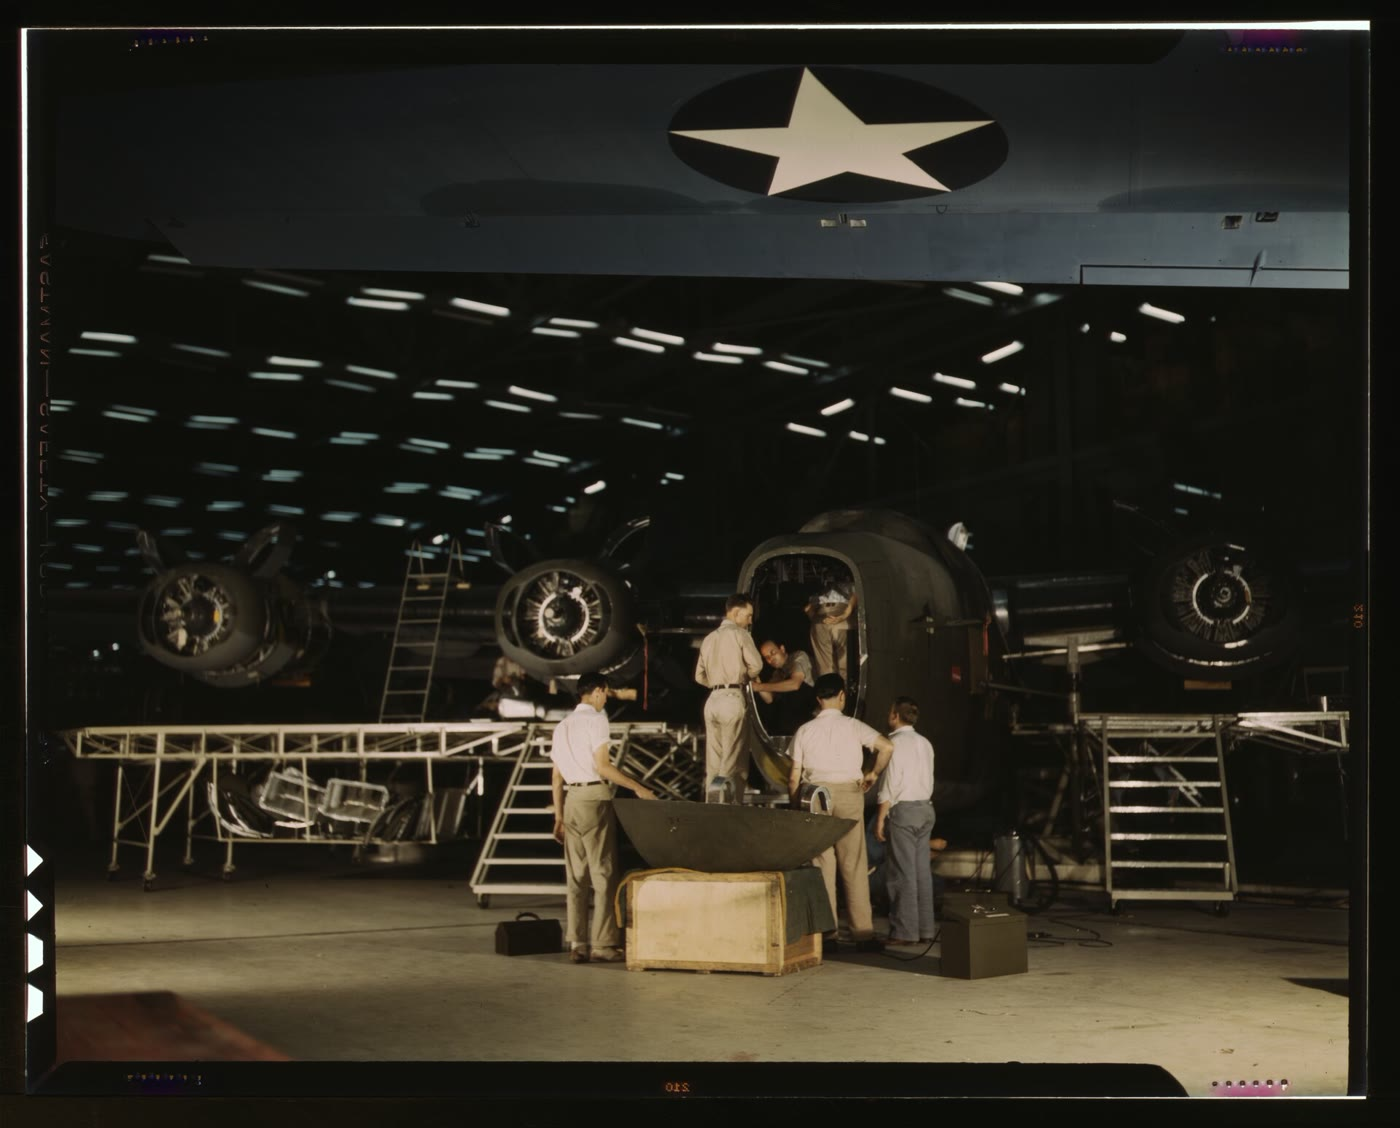
\includegraphics[width=0.58\linewidth]{images/book2/photos/g10-ppf-aircraft-assembly-1942.jpg}

{\small Workers fit a nose door to a C-87 transport plane at the end of the assembly line of an aircraft plant in Fort Worth, Texas, October 1942.}
\end{omfigure}

\section{Moving the frontier}\label{sec:g10:production-possibility-frontier:moving}

The frontier is drawn for given factors and a given technology. When either changes, the frontier
moves.
\begin{itemize}
\item \textbf{More factors.} More workers, more machines or more land let the economy produce more of
  both goods: the whole frontier moves outward.
\item \textbf{Better technology in one good.} A new loom that halves the hours needed for a roll of
  cloth raises the most cloth that can be made, but not the most grain: the frontier moves outward
  along the cloth axis and stays where it was on the grain axis.
\end{itemize}

\begin{example}[A new loom in the North Valley]\label{ex:g10:production-possibility-frontier:loom}
Suppose a new loom cuts the time for a roll of cloth in the North Valley from 2 hours to 1. The North
can now make \num{1200} rolls instead of 600, and a tonne of grain there now costs $3/1 = 3$ rolls of
cloth instead of 1.5. The two valleys together can make $1200 + 1200 = 2400$ rolls with no grain, and
still at most 600 tonnes of grain with no cloth. The North is still the cheaper place for grain (3 rolls
a tonne against 6), so the kink stays at 400 tonnes, now with $2400 - 400 \times 3 = 1200$ rolls. The
new frontier joins $(0, 2400)$, $(400, 1200)$ and $(600, 0)$.
\end{example}

\begin{omfigure}
\begin{tikzpicture}[econ, x=0.011cm, y=0.0024cm]
\draw[econ axes] (0,2700) node[left, font=\small] {cloth $C$ (rolls)} |- (760,0) node[below left=12pt and 0pt, font=\small] {grain $G$ (tonnes)};
\draw[ppf] (0,1800) -- (400,1200) -- (600,0);
\draw[ppf, shifted, omThm] (0,2400) -- (400,1200);
\foreach \y in {1200,1800,2400} \draw (0,\y) -- (-8,\y) node[left, font=\footnotesize] {\num{\y}};
\foreach \x in {200,400,600} \draw (\x,0) -- (\x,-45) node[below, font=\footnotesize] {\x};
\draw[phase arrow] (60,1740) -- (60,2190);
\node[font=\footnotesize, anchor=west] at (140,2150) {after the new loom};
\node[font=\footnotesize, anchor=west] at (420,1350) {unchanged from here};
\end{tikzpicture}

{\small A new loom in the North Valley moves the joint frontier outward along the cloth axis (dashed).
The most grain the valleys can produce, 600 tonnes, does not change, and beyond the kink the frontier
is the same as before, because there the North already makes only grain.}
\end{omfigure}

\begin{remark}[A choice today moves the frontier tomorrow]\label{rem:g10:production-possibility-frontier:invest}
Replace grain and cloth by consumer goods and capital goods (machines, buildings, tools). A society that
chooses a point with more capital goods this year consumes less now, but it has more machines next year,
so its frontier next year lies further out. The choice of a point on this year's frontier is also a
choice of where next year's frontier will be. The grade 12 chapters on saving, investment and growth
measure how strong this link is.
\end{remark}

\section{Exercises}

\begin{exercise}[$\star$]\label{exo:g10:production-possibility-frontier:1}
Read the opening chart. In the United States, what were the indices of output per person and of
consumption per person in 1944? In the United Kingdom, in 1943?
\end{exercise}

\begin{exercise}[$\star$]\label{exo:g10:production-possibility-frontier:2}
Read the opening chart. In which year after the war did American consumption per person first exceed
125? What happened to output per person between 1944 and 1947?
\end{exercise}

\begin{exercise}[$\star$]\label{exo:g10:production-possibility-frontier:3}
For the North Valley ($3G + 2C \le 1200$), say whether each combination is on the frontier, inside it,
or out of reach: (a) 100 tonnes of grain and 450 rolls of cloth; (b) 300 tonnes and 200 rolls; (c) 50
tonnes and 500 rolls.
\end{exercise}

\begin{exercise}[$\star$]\label{exo:g10:production-possibility-frontier:4}
A village has 600 hours of work a week. A basket of fish takes 2 hours and a basket of fruit 3 hours.
Write the equation of its frontier with fruit on the vertical axis, and give the most fish and the most
fruit it can produce.
\end{exercise}

\begin{exercise}[$\star$]\label{exo:g10:production-possibility-frontier:5}
For the village of \cref{exo:g10:production-possibility-frontier:4}, what is the opportunity cost of a
basket of fish, in baskets of fruit? And of a basket of fruit, in baskets of fish?
\end{exercise}

\begin{exercise}[$\star\star$]\label{exo:g10:production-possibility-frontier:6}
Two islands produce fish and fruit. The East Island has 600 hours a week, with 2 hours per basket of
fish and 3 hours per basket of fruit. The West Island has 600 hours, with 4 hours per basket of fish and
2 hours per basket of fruit. Find the most fish and the most fruit the two islands can produce together,
and the kink of their joint frontier. Draw the frontier.
\end{exercise}

\begin{exercise}[$\star\star$]\label{exo:g10:production-possibility-frontier:7}
On the joint frontier of the two valleys (\cref{ex:g10:production-possibility-frontier:two}), how much
cloth is given up when grain rises from 100 to 300 tonnes? From 400 to 500 tonnes? Explain the
difference.
\end{exercise}

\begin{exercise}[$\star\star$]\label{exo:g10:production-possibility-frontier:8}
A tractor arrives in the South Valley and cuts the time for a tonne of grain there from 6 hours to 4.
Predict how the joint frontier of the two valleys changes: which end moves, by how much, and does the
kink move?
\end{exercise}

\begin{exercise}[$\star\star$]\label{exo:g10:production-possibility-frontier:9}
The two valleys produce 300 tonnes of grain with the North Valley making 200 tonnes and the South 100.
How much cloth do they make? How much could they make with the same 300 tonnes of grain? Is the first
combination \omterm{def:g10:production-possibility-frontier:productive-efficiency}{productively efficient}?
\end{exercise}

\begin{exercise}[$\star\star$]\label{exo:g10:production-possibility-frontier:10}
On a smooth bowed frontier, the combinations $(10, 95)$, $(20, 85)$ and $(30, 70)$ are three points
(grain, cloth). Compute the average opportunity cost of a unit of grain between the first two points and
between the last two. Do these numbers agree with the \omterm{def:g10:production-possibility-frontier:increasing-cost}{law of increasing opportunity cost}?
\end{exercise}

\begin{exercise}[$\star\star$]\label{exo:g10:production-possibility-frontier:11}
Read the second chart. By how many percentage points did unemployment fall between 1939 and 1944 in each
country? Use the answer to explain why the two countries paid so differently for their war output.
\end{exercise}

\begin{exercise}[$\star\star\star$]\label{exo:g10:production-possibility-frontier:12}
Someone claims that in a certain country the opportunity cost of food rises as more food is produced.
What observation, over a period in which the factors and the technology stayed the same, would contradict
this claim? Why must the factors and the technology have stayed the same?
\end{exercise}

\begin{exercise}[$\star\star\star$]\label{exo:g10:production-possibility-frontier:13}
Prove that if two regions have the same opportunity cost of grain, their joint frontier is a straight
line, with no kink.
\end{exercise}

\begin{exercise}[$\star\star\star$]\label{exo:g10:production-possibility-frontier:14}
Add a third valley to \cref{ex:g10:production-possibility-frontier:two}: the West Valley, with 600 hours a
week, 2 hours per tonne of grain and 3 hours per roll of cloth. Find the joint frontier of the three
valleys: its two ends, its kinks and the slope of each piece.
\end{exercise}

\begin{exercise}[$\star\star\star$]\label{exo:g10:production-possibility-frontier:15}
An economy makes consumer goods $c$ and machines $m$ with the frontier $c + 2m = 100$ this year. Each
machine made this year moves next year's frontier outward: next year it is $c + 2m = 100 + 3m_1$, where
$m_1$ is the number of machines made this year. Compare two plans: (a) $m_1 = 0$ this year; (b) $m_1 =
20$ this year. In each plan, how many consumer goods are made this year, and how many can be made next
year if next year no machines are made? Which plan gives more consumer goods over the two years
together?
\end{exercise}

\section{Problem: Brenland's Harvest Campaign}

\begin{problem}[{Weekend problem --- three regions, one target, and the cost of the last tonne}]
\label{pb:g10:production-possibility-frontier:1}
Brenland has three farming regions. Each produces grain and cloth with its own hours of work and its own
skills (invented numbers; grain in thousands of tonnes, cloth in thousands of metres, hours in thousands
a year):

\begin{center}
\small
\begin{tabular}{lrrr}
\toprule
region & hours available & hours per tonne of grain & hours per metre of cloth \\
\midrule
Hills & 300 & 10 & 2 \\
River & 400 & 4 & 4 \\
Plain & 300 & 2 & 6 \\
\bottomrule
\end{tabular}
\end{center}

\noindent The government announces a harvest campaign: grain is to rise from \num{200000} to
\num{260000} tonnes a year, with the regions organised efficiently before and after.

\medskip
\noindent\textbf{Part I --- The three regions.}
\begin{enumerate}
\item For each region, compute the most grain it can produce (with no cloth) and the most cloth (with no
  grain).
\item For each region, compute the opportunity cost of one tonne of grain, in metres of cloth.
\item Which region has the lowest opportunity cost of grain? Which has the lowest opportunity cost of
  cloth?
\item Write the frontier of the River region as an equation, with cloth $C$ as a function of grain $G$.
\end{enumerate}

\medskip
\noindent\textbf{Part II --- The joint frontier.}
\begin{enumerate}[resume]
\item What are the two ends of Brenland's joint frontier?
\item Starting from all cloth, in which order should the regions switch to grain? Justify.
\item Find the two kinks of the joint frontier.
\item Give the slope of each of the three pieces.
\item Draw the joint frontier.
\end{enumerate}

\medskip
\noindent\textbf{Part III --- The campaign.}
\begin{enumerate}[resume]
\item How much cloth does Brenland produce, on the frontier, with \num{200000} tonnes of grain? Which
  region produces both goods?
\item How much cloth does it produce with \num{260000} tonnes?
\item What is the total cost of the campaign, in metres of cloth? What is the average cost of each extra
  tonne?
\item A careless plan reaches \num{260000} tonnes by ordering the Hills to produce only grain, the River
  region to produce \num{100000} tonnes, and the Plain to produce the rest. How much cloth does Brenland
  make then? How much cloth is wasted compared with the efficient plan?
\item Where does the careless plan's point lie, compared with the frontier? Name the definition it fails.
\end{enumerate}

\medskip
\noindent\textbf{Part IV --- The last tonne.}
\begin{enumerate}[resume]
\item What is the opportunity cost of the first \num{1000} tonnes of grain Brenland produces, starting from
  all cloth?
\item What is the opportunity cost of the last \num{1000} tonnes, on the way to the most grain Brenland
  can produce?
\item By what factor is the last tonne dearer than the first? Which law does this illustrate?
\item A new loom cuts the hours per metre of cloth in the Hills from 2 to 1. Which end of the joint
  frontier moves, and to where?
\item With the new loom, what is the opportunity cost of the last \num{1000} tonnes of grain now?
\item State the result of the problem: the opportunity cost of the last \num{1000} tonnes of grain, in
  metres of cloth, before the new loom, and compare it with the cost of the campaign's average tonne.
\end{enumerate}
\end{problem}
